\documentclass[12pt]{article}
\usepackage{amsmath,amssymb,amsthm,fullpage,bm,graphicx,accents}
\usepackage{listings,lstautogobble,color,subcaption}
\usepackage{hyperref}
\usepackage{natbib}


%%%%%%%%%%%%%%%%%%%%%%%%%%%%%%%%%%%%%%%%%%
% Custom commands                        %
%%%%%%%%%%%%%%%%%%%%%%%%%%%%%%%%%%%%%%%%%%

\newcommand{\vc}[1]{\boldsymbol{#1}}
\newcommand{\adj}[1]{\frac{d J}{d #1}}
\newcommand{\chain}[2]{\adj{#2} = \adj{#1}\frac{d #1}{d #2}}

% mathcal
\newcommand{\Ac}{\mathcal{A}}
\newcommand{\Bc}{\mathcal{B}}
\newcommand{\Cc}{\mathcal{C}}
\newcommand{\Dc}{\mathcal{D}}
\newcommand{\Ec}{\mathcal{E}}
\newcommand{\Fc}{\mathcal{F}}
\newcommand{\Gc}{\mathcal{G}}
\newcommand{\Hc}{\mathcal{H}}
\newcommand{\Ic}{\mathcal{I}}
\newcommand{\Jc}{\mathcal{J}}
\newcommand{\Kc}{\mathcal{K}}
\newcommand{\Lc}{\mathcal{L}}
\newcommand{\Mc}{\mathcal{M}}
\newcommand{\Nc}{\mathcal{N}}
\newcommand{\Oc}{\mathcal{O}}
\newcommand{\Pc}{\mathcal{P}}
\newcommand{\Qc}{\mathcal{Q}}
\newcommand{\Rc}{\mathcal{R}}
\newcommand{\Sc}{\mathcal{S}}
\newcommand{\Tc}{\mathcal{T}}
\newcommand{\Uc}{\mathcal{U}}
\newcommand{\Vc}{\mathcal{V}}
\newcommand{\Wc}{\mathcal{W}}
\newcommand{\Xc}{\mathcal{X}}
\newcommand{\Yc}{\mathcal{Y}}
\newcommand{\Zc}{\mathcal{Z}}

% mathbb
\newcommand{\Ab}{\mathbb{A}}
\newcommand{\Bb}{\mathbb{B}}
\newcommand{\Cb}{\mathbb{C}}
\newcommand{\Db}{\mathbb{D}}
\newcommand{\Eb}{\mathbb{E}}
\newcommand{\Fb}{\mathbb{F}}
\newcommand{\Gb}{\mathbb{G}}
\newcommand{\Hb}{\mathbb{H}}
\newcommand{\Ib}{\mathbb{I}}
\newcommand{\Jb}{\mathbb{J}}
\newcommand{\Kb}{\mathbb{K}}
\newcommand{\Lb}{\mathbb{L}}
\newcommand{\Mb}{\mathbb{M}}
\newcommand{\Nb}{\mathbb{N}}
\newcommand{\Ob}{\mathbb{O}}
\newcommand{\Pb}{\mathbb{P}}
\newcommand{\Qb}{\mathbb{Q}}
\newcommand{\Rb}{\mathbb{R}}
\newcommand{\Sb}{\mathbb{S}}
\newcommand{\Tb}{\mathbb{T}}
\newcommand{\Ub}{\mathbb{U}}
\newcommand{\Vb}{\mathbb{V}}
\newcommand{\Wb}{\mathbb{W}}
\newcommand{\Xb}{\mathbb{X}}
\newcommand{\Yb}{\mathbb{Y}}
\newcommand{\Zb}{\mathbb{Z}}

% mathbf lowercase
\newcommand{\av}{\mathbf{a}}
\newcommand{\bv}{\mathbf{b}}
\newcommand{\cv}{\mathbf{c}}
\newcommand{\dv}{\mathbf{d}}
\newcommand{\ev}{\mathbf{e}}
\newcommand{\fv}{\mathbf{f}}
\newcommand{\gv}{\mathbf{g}}
\newcommand{\hv}{\mathbf{h}}
\newcommand{\iv}{\mathbf{i}}
\newcommand{\jv}{\mathbf{j}}
\newcommand{\kv}{\mathbf{k}}
\newcommand{\lv}{\mathbf{l}}
\newcommand{\mv}{\mathbf{m}}
\newcommand{\nv}{\mathbf{n}}
\newcommand{\ov}{\mathbf{o}}
\newcommand{\pv}{\mathbf{p}}
\newcommand{\qv}{\mathbf{q}}
\newcommand{\rv}{\mathbf{r}}
\newcommand{\sv}{\mathbf{s}}
\newcommand{\tv}{\mathbf{t}}
\newcommand{\uv}{\mathbf{u}}
\newcommand{\vv}{\mathbf{v}}
\newcommand{\wv}{\mathbf{w}}
\newcommand{\xv}{\mathbf{x}}
\newcommand{\yv}{\mathbf{y}}
\newcommand{\zv}{\mathbf{z}}

% mathbf uppercase
\newcommand{\Av}{\mathbf{A}}
\newcommand{\Bv}{\mathbf{B}}
\newcommand{\Cv}{\mathbf{C}}
\newcommand{\Dv}{\mathbf{D}}
\newcommand{\Ev}{\mathbf{E}}
\newcommand{\Fv}{\mathbf{F}}
\newcommand{\Gv}{\mathbf{G}}
\newcommand{\Hv}{\mathbf{H}}
\newcommand{\Iv}{\mathbf{I}}
\newcommand{\Jv}{\mathbf{J}}
\newcommand{\Kv}{\mathbf{K}}
\newcommand{\Lv}{\mathbf{L}}
\newcommand{\Mv}{\mathbf{M}}
\newcommand{\Nv}{\mathbf{N}}
\newcommand{\Ov}{\mathbf{O}}
\newcommand{\Pv}{\mathbf{P}}
\newcommand{\Qv}{\mathbf{Q}}
\newcommand{\Rv}{\mathbf{R}}
\newcommand{\Sv}{\mathbf{S}}
\newcommand{\Tv}{\mathbf{T}}
\newcommand{\Uv}{\mathbf{U}}
\newcommand{\Vv}{\mathbf{V}}
\newcommand{\Wv}{\mathbf{W}}
\newcommand{\Xv}{\mathbf{X}}
\newcommand{\Yv}{\mathbf{Y}}
\newcommand{\Zv}{\mathbf{Z}}

% bold greek lowercase
\newcommand{\alphav     }{\boldsymbol \alpha     }
\newcommand{\betav      }{\boldsymbol \beta      }
\newcommand{\gammav     }{\boldsymbol \gamma     }
\newcommand{\deltav     }{\boldsymbol \delta     }
\newcommand{\epsilonv   }{\boldsymbol \epsilon   }
\newcommand{\varepsilonv}{\boldsymbol \varepsilon}
\newcommand{\zetav      }{\boldsymbol \zeta      }
\newcommand{\etav       }{\boldsymbol \eta       }
\newcommand{\thetav     }{\boldsymbol \theta     }
\newcommand{\varthetav  }{\boldsymbol \vartheta  }
\newcommand{\iotav      }{\boldsymbol \iota      }
\newcommand{\kappav     }{\boldsymbol \kappa     }
\newcommand{\varkappav  }{\boldsymbol \varkappa  }
\newcommand{\lambdav    }{\boldsymbol \lambda    }
\newcommand{\muv        }{\boldsymbol \mu        }
\newcommand{\nuv        }{\boldsymbol \nu        }
\newcommand{\xiv        }{\boldsymbol \xi        }
\newcommand{\omicronv   }{\boldsymbol \omicron   }
\newcommand{\piv        }{\boldsymbol \pi        }
\newcommand{\varpiv     }{\boldsymbol \varpi     }
\newcommand{\rhov       }{\boldsymbol \rho       }
\newcommand{\varrhov    }{\boldsymbol \varrho    }
\newcommand{\sigmav     }{\boldsymbol \sigma     }
\newcommand{\varsigmav  }{\boldsymbol \varsigma  }
\newcommand{\tauv       }{\boldsymbol \tau       }
\newcommand{\upsilonv   }{\boldsymbol \upsilon   }
\newcommand{\phiv       }{\boldsymbol \phi       }
\newcommand{\varphiv    }{\boldsymbol \varphi    }
\newcommand{\chiv       }{\boldsymbol \chi       }
\newcommand{\psiv       }{\boldsymbol \psi       }
\newcommand{\omegav     }{\boldsymbol \omega     }

% bold greek uppercase
\newcommand{\Gammav     }{\boldsymbol \Gamma     }
\newcommand{\Deltav     }{\boldsymbol \Delta     }
\newcommand{\Thetav     }{\boldsymbol \Theta     }
\newcommand{\Lambdav    }{\boldsymbol \Lambda    }
\newcommand{\Xiv        }{\boldsymbol \Xi        }
\newcommand{\Piv        }{\boldsymbol \Pi        }
\newcommand{\Sigmav     }{\boldsymbol \Sigma     }
\newcommand{\Upsilonv   }{\boldsymbol \Upsilon   }
\newcommand{\Phiv       }{\boldsymbol \Phi       }
\newcommand{\Psiv       }{\boldsymbol \Psi       }
\newcommand{\Omegav     }{\boldsymbol \Omega     }

\newcommand{\argmin}{\mathop{\mathrm{argmin}}}
\newcommand{\argmax}{\mathop{\mathrm{argmax}}}

\title{Toward Understanding Long Sequence Time Series Forecasting via Transformers}
\author{Ethan Wu, Donghan Yu, Ruohong Zhang, Yiming Yang}
\date{\today}

\begin{document}
\maketitle
\begin{abstract}
Making long sequence forecasting on time series involves a number of modeling challenges. 
Nonetheless, Transformer architecture inspires recent progress in this domain. 
In this report, we focus on two major advancements: non-autoregressive decoding and Autoformer architecture. 
A number of experiments on real-world and synthetic datasets are performed to verify their superior performance and investigate their working mechanism. 
In addition, the benefits and drawbacks of different methods are discussed. 
We summarize our findings and interpretations in the final discussion. \footnote{The code is available at: \href{https://github.com/yongyi-wu/lstf}{https://github.com/yongyi-wu/lstf}.}
\end{abstract}

\section{Introduction}
Time series has long been a heated research domain for the machine learning community. 
Successful modeling of temporal patterns has profound applications in finance, logistics, natural sciences, etc. 
The forecasting task can be formulated as predicting observations in the future $\Xv_\text{output} \in \Rb^{L_\text{target} \times d}$ based on the observations up until now $\Xv_\text{input} \in \Rb^{L_\text{input} \times d}$. 
However, non-stationarity in many real-world scenarios complicates the task. 
Another challenge arises due to multivariate signal ($d > 1$), which entails the consideration of spatial relationship. 
Finally, long sequence forecasting (large $L_\text{target}$), which involves predictions for tens or hundreds of future timestamps, requires the ability to capture long-term dependencies. 

The neural network approach to time series forecasting was once dominated by Recurrent Nueral Networks (\citet{https://doi.org/10.48550/arxiv.1703.07015}).  
More recently, however, Transformer due to \citet{https://doi.org/10.48550/arxiv.1706.03762} has created a new paradigm for the deep learning community. 
The architecture has achieved record-breaking successes in a number of Computer Vision and Natural Language Processing tasks. 
A subsequent question is how we can adopt this architecture to tackle challenges in time series forecasting. 
\citet{https://doi.org/10.48550/arxiv.1907.00235} introduces the LogSparse Transformer to reduce the asymptotic cost of the multihead attention. 
The Informer due to \citet{https://doi.org/10.48550/arxiv.2012.07436} leverages non-autoregressive decoding and renovates the attention mechanism again. 
By injecting stronger inductive biases, \citet{https://doi.org/10.48550/arxiv.2106.13008} replaces the attention and layer normalization (\citet{https://doi.org/10.48550/arxiv.1607.06450}) modules by autocorrelation and decomposition modules, respectively. 
While retaining the decomposition scheme, FEDformer by \citet{https://doi.org/10.48550/arxiv.2201.12740} shifts to modeling frequency-domain signals instead. 

Of all recent progress, Informer (\citet{https://doi.org/10.48550/arxiv.2012.07436}) and Autoformer (\citet{https://doi.org/10.48550/arxiv.2106.13008}) have shown most dramatic improvement compared to previous methods, which motivate the experiments presented in this report. 
In particular, we conduct comprehensive ablation studies on real and synthetic datasets to: \begin{itemize}
    \item Verify the superior performance of Informer's non-autoregressive decoding versus the autoregressive counterpart; 
    \item Investigate the inductive biases in Autoformer's autocorrelation module and decomposition module. 
\end{itemize}


\section{Non-Autoregressive Decoding}
\subsection{Architecture}
Informer (\citet{https://doi.org/10.48550/arxiv.2012.07436}) is the first Transformer variant that exploites non-autoregressive decoding (termed \textit{generative inference} in the paper) for time series forecasting. 
The key idea is to predict $L_\text{target}$ future timestamps in just one forward pass and thus save inference time. 
In this section, we focus on vanilla Transformers (\citet{https://doi.org/10.48550/arxiv.1706.03762}) with different decoding schemes. 

\subsubsection{Multihead Attention}
The attention mechanism follows the vanilla multihead attention. 
Within each head, the output is computed by $$\text{Attention}(\Qv, \Kv, \Vv) = \text{softmax}(\frac{\Qv\Kv^T}{\sqrt{d}}) \Vv.$$
Overall, the output is $\text{Multihead}(\Qv, \Kv, \Vv) = [\text{head}_1 \| \text{head}_2 \| \cdots \| \text{head}_h]\Wv^O$, where we define $\text{head}_i = \text{Attention}(\Qv\Wv_i^Q, \Kv\Wv_i^K, \Vv\Wv_i^V)$. 
Here, $\|$ is the concatenation operator and $\Wv$'s are projection matrices of appropriate shapes. 

\subsubsection{Decoder}
The autoregressive decoder follows the design of seq2seq Transformer models. 
In a long sequence forecasting setting, when predicting values $X_{j, *} \in \Rb^{d}$ at timestamp $j$, we concatenate all previous predictions $\hat{\Xv}_{<j, *} \in \Rb^{(j - 1) \times d}$ and feed them into the model.  
Notice that this decoding scheme is inherently sequential and hence can be extremely slow during inference. 
Moreover, the model is vulnerable to the training-testing distribution shift due to teacher-forced training (\citet{6795228}). 

On the other hand, non-autoregressive decoder forecasts in parallel. 
The layout of decoder input is shown in Figure \ref{fig:nonauto_input}, where the dark green blocks are (optionally) previous observations that create \textit{context} for decoding, 
the white zero blocks are placeholders where predictions will be made, 
and the light green blocks are positional and temporal embeddings which are intact. 
Finally, a triangular causal mask is applied to decoder's self attention module so that each timestamp can attend to previous observations only. 

\begin{figure}
    \centering
    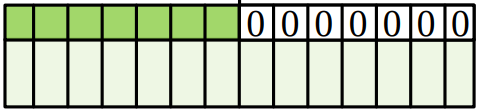
\includegraphics[width=0.4\textwidth]{img/nonauto_input.png}
    \caption{Input to a non-autoregressive decoder.}
    \label{fig:nonauto_input}
\end{figure}

\subsection{Experiments}

While the Informer paper (\citet{https://doi.org/10.48550/arxiv.2012.07436}) does contain an ablation study on the non-autoregressive decoding, only two prediction lengths $L_\text{target}$ are examined and the authors did not decouple the influence of the noval attention module. 
To verify the superiority of a non-autoregressive decoder, we run more experiments on six real-world benchmarks and observe expected results. 

Interestingly, we also notice that the decoder taking input as Figure \ref{fig:nonauto_input} is sufficient to perform forecasting. 
Therefore, we remove encoder and evaluate the \texttt{Decoder-Only} model as well. 

\subsubsection{Datasets}\label{benchmarks}

We use six real-world dataset that are popular in time series research community: \begin{itemize}
    \item \texttt{ETT}(\citet{https://doi.org/10.48550/arxiv.2012.07436}): This dataset is related to electric power deployment. The data is 7-dimensional plus a timestamp. 
    The sampling rate of \texttt{ETTh1} is 1 hour and of \texttt{ETTm2} is 15 minutes. 
    \texttt{ETTh1} has 14k observations in total, whereas \texttt{ETTm2} has 70k observations in total. 
    \item \texttt{Electricity}\footnote{https://archive.ics.uci.edu/ml/datasets/ElectricityLoadDiagrams20112014}: It contains electricity consumption of 321 clients. The sampling rate is 1 hour. There are 26k observations in total. 
    \item \texttt{Exchange}(\citet{https://doi.org/10.48550/arxiv.1703.07015}): It documents daily exchange rate across 7 countries. There are 8k observations in total. 
    \item \texttt{Traffic}\footnote{http://pems.dot.ca.gov/}: This is a collection of road occupancy rates of 862 San Francisco Bay area freeways. The sampling rate is 1 hour. There are 18k observations in total. 
    \item \texttt{Weather}\footnote{https://www.bgc-jena.mpg.de/wetter/}: This is local climatological data from 2010 to 2013 of the United States. The data is 20-dimensional plus a timestamp. 
    The sampling rate is 1 hour. There are 50k observations in total. 
    \item \texttt{ILI}\footnote{https://gis.cdc.gov/grasp/fluview/fluportaldashboard.html}: The dataset contains the percentage of patients with influenza-like illness from 2002 to 2021. 
    The data is 7-dimensional plus the timestamp with a 7-day sampling rate. There are 967 observations in total. 
\end{itemize}

\subsubsection{Results}
Figure \ref{fig:mse_nonauto} shows the mean square errors of forecasting results on different test datasets with varied prediction lengths. 
The lower the bar, the better the model. 
Overall, non-autoregressive decoding performs on par with, if not better than, autoregressive decoding. 
The gap is especially large in \texttt{Electricity} and \texttt{Traffic} datasets. 
A possible reason is that time series forecasting relies more on an understanding of large-scale pattern; 
instead, the dependencies on previous one timestamp or two are rather weak. 
Therefore, autoregression does not bring about significant advantage. 

\begin{figure}
    \centering
    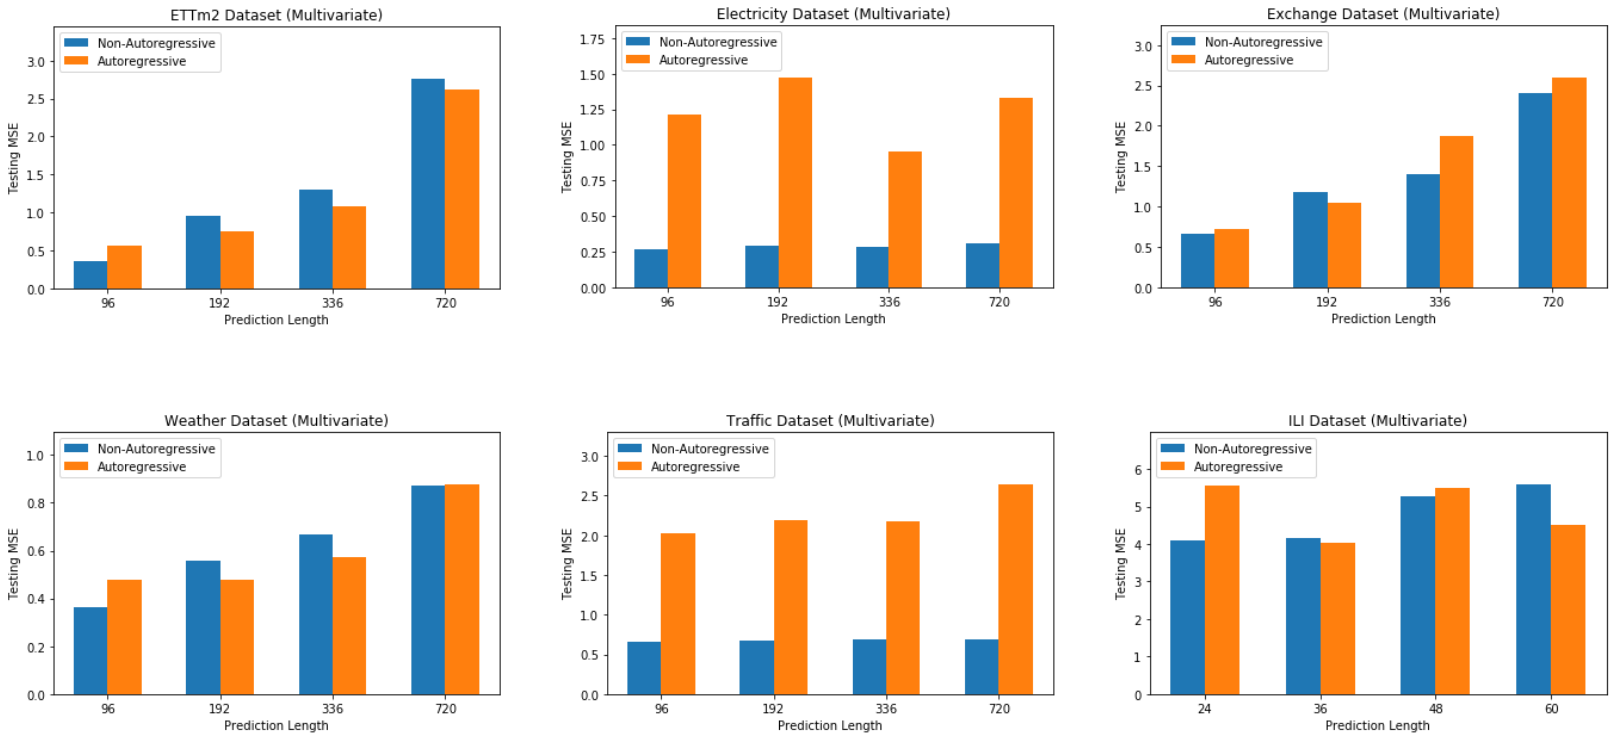
\includegraphics[width=\textwidth]{img/mse_nonauto.png}
    \caption{Mean square errors of autoregressive versus non-autoregressive decoding.}
    \label{fig:mse_nonauto}
\end{figure}

Taking the inference speed into account, Figure \ref{fig:nonauto_time} indicates that autoregressive decoding is an undisirable choice for sure. 
Interestingly, while \citet{https://doi.org/10.48550/arxiv.2012.07436} claims that Informer improves the asymptotic cost of the attention mechanism, empirically vanilla attention with non-autoregressive decoding takes even smaller amount of time. 
This result highlights the discrepancy between the asymptotic analysis and wall-clock time. 
Meanwhile, it reinforces the necessity of incorporating non-autoregressive decoding scheme into Transformer variants for the long sequence time series forecasting. 

\begin{figure}
    \centering
    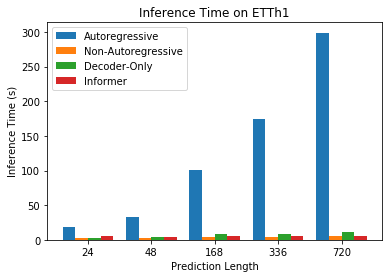
\includegraphics[width=0.6\textwidth]{img/nonauto_time.png}
    \caption{Inference speed measured by second on the \texttt{ETTh1} test dataset.}
    \label{fig:nonauto_time}
\end{figure}

As mentioned previously, we also evaluate a vanilla Transformer without an encoder, since the non-autoregressive decoder is theoretically with contextualized input (Figure \ref{fig:nonauto_input}) is sufficient in this setting. 
Figure \ref{fig:mse_noenc} compares results with state-of-the-art Transformer variants. 
Although the \texttt{Decoder-Only} model has achieved competitive performance against Informer, it falls short of more recent models equipped with the decomposition module. 
Moreover, we found empirically that \texttt{Decoder-Only} is insensitive as we scale up the model parameters. 
Thus, while removing the encoder can be a promising way to reduce model size robustly, it fails to generate significant improvement. 
The hope lies in the architecture innovation. 

\begin{figure}
    \centering
    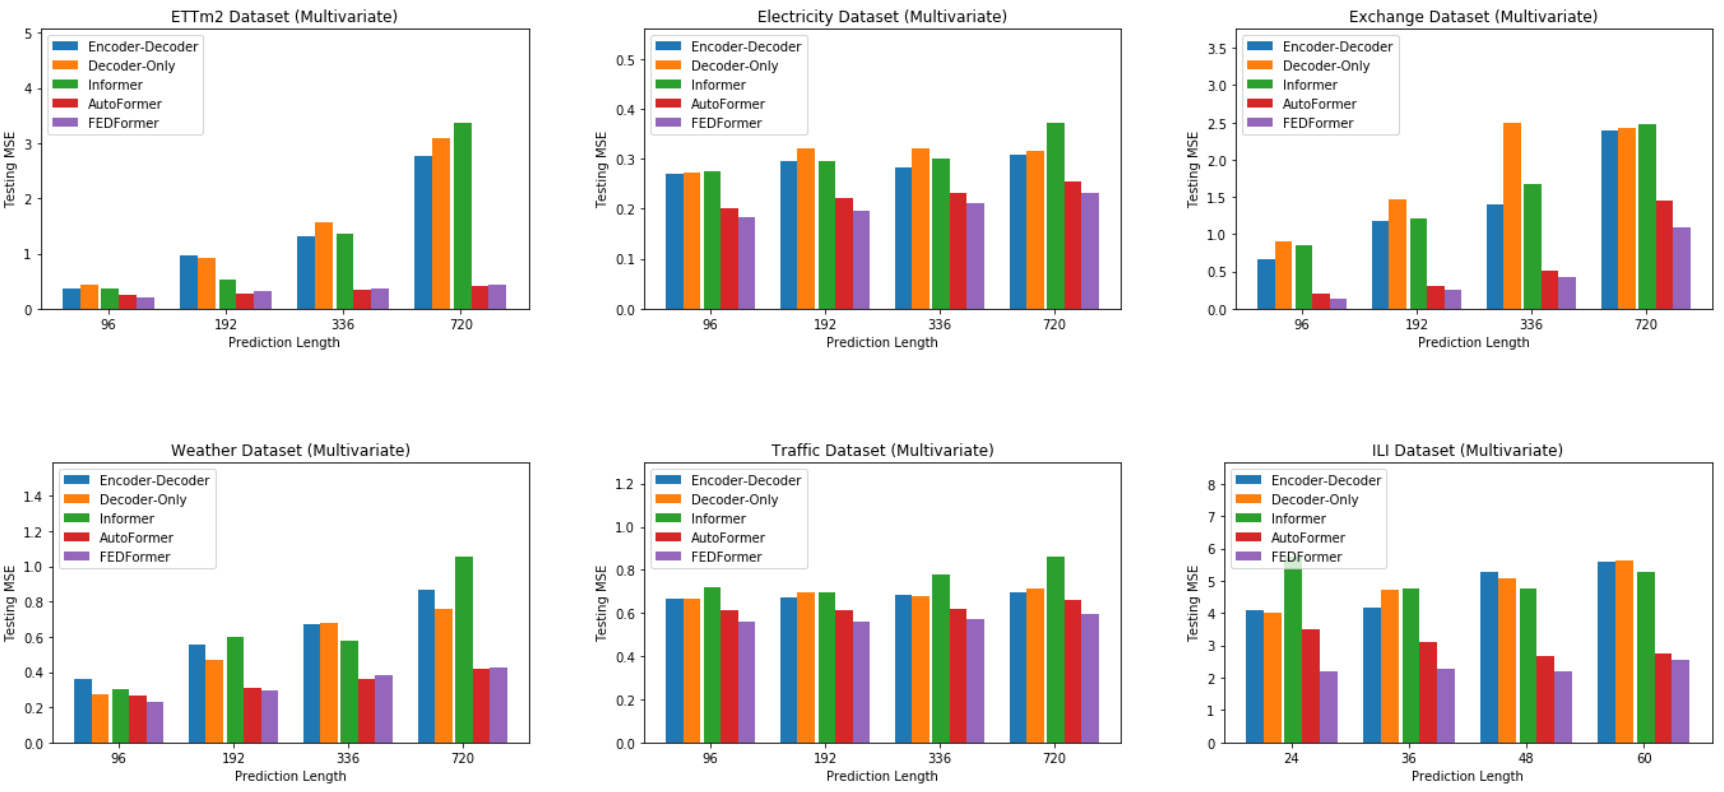
\includegraphics[width=\textwidth]{img/mse_noenc.png}
    \caption{Mean square errors of Transformers with and without encoder as well as state-of-the-art variants.}
    \label{fig:mse_noenc}
\end{figure}



\section{Autoformer Architecture}
\subsection{Architecture}
Autoformer (\citet{https://doi.org/10.48550/arxiv.2106.13008}) makes substantial modifications to the building blocks of Transformer. 
As shown in Figure \ref{fig:autoformer}, the multihead attention module is replaced by the autocorrelation module, and layer normalization module by decomposition module. 
The idea is to emulate the traditional seasonal-trend decomposition (\citet{cleveland90}) while leverage the flexibility of neural networks to model periodic patterns. 

\begin{figure}
    \centering
    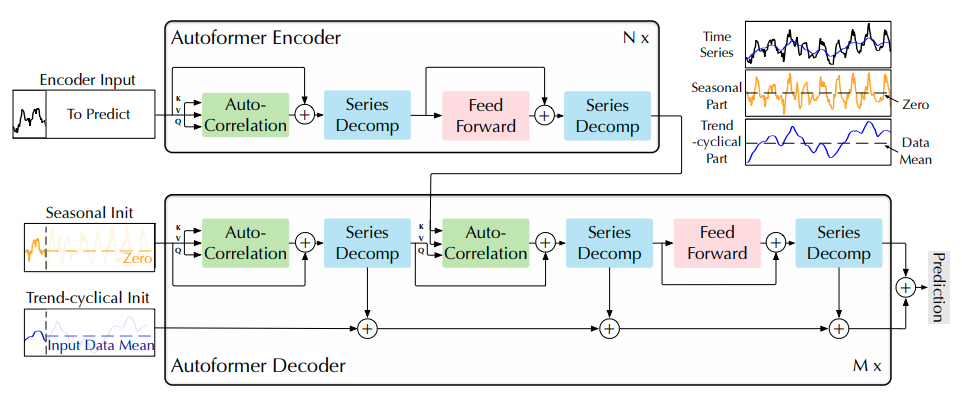
\includegraphics[width=0.8\textwidth]{img/autoformer.png}
    \caption{A visualization of Autoformer architecture.}
    \label{fig:autoformer}
\end{figure}

\subsubsection{Decomposition Module}
The module aims at decomposing the input signal $X \in \Rb^L$ into trend $T \in \Rb^L$ and seasonality $S \in \Rb^L$ such that $X = T + S$. 
The trend is expected to contain long-term non-stationary changes, whereas seasonality is more concerned about cyclical patterns. 
To this end, we just compute moving average (i.e. perform average pooling) along the temporal domain to obtain the trend, and substact it element-wise to get seasonality. 
Mathematically, we have \begin{align*}
    T &= \text{AvgPool}(X) & S &= X - T.
\end{align*}

Notice in Figure \ref{fig:autoformer} that the input into the decoder gets decomposed in the beginning, which, we hypothesize, gives an appropriate \textit{baseline} for later forecasting. 
As noted by \citet{https://doi.org/10.48550/arxiv.2202.07125}, the decomposition mechanism indeed boosts all Transformer variants' performance significantly. 
These ideas will be revisited in our experiments. 

\subsubsection{Autocorrelation Module}
This module emulates the idea of autocorrelation to compute sequence-level similarities in hope of capturing period-based dependencies. 
More formally, the similarity between a query sequence $Q \in \Rb^{L}$ and a $\tau$-delayed key sequence $K \in \Rb^{L}$ is defined as $$R_{Q, K}(\tau) = \sum_{t = 1}^L Q_tK_{t - \tau}.$$
The intuition is that $R_{Q, K}(\tau)$ will be large in magnitude if two sequences are similar and have period $\tau$. 
To optimize memory and speed consumptions, only top-$k$ different $\tau$'s that give high $R_{Q, K}(\tau)$ are selected and normalized by \texttt{softmax} to be attention weights $\{\alpha_{\tau_i}\}_{i = 1}^k$. 
Finally, the output is the linear combination of $k$ different wrap-arounded (i.e. \texttt{Roll}-ed) value sequences $V \in \Rb^{L}$: $\sum_{i = 1}^k \alpha_{\tau_i} \text{Roll}(V, \tau_i)$ (see Figure \ref{fig:autocorrelation}). 

\begin{figure}
    \centering
    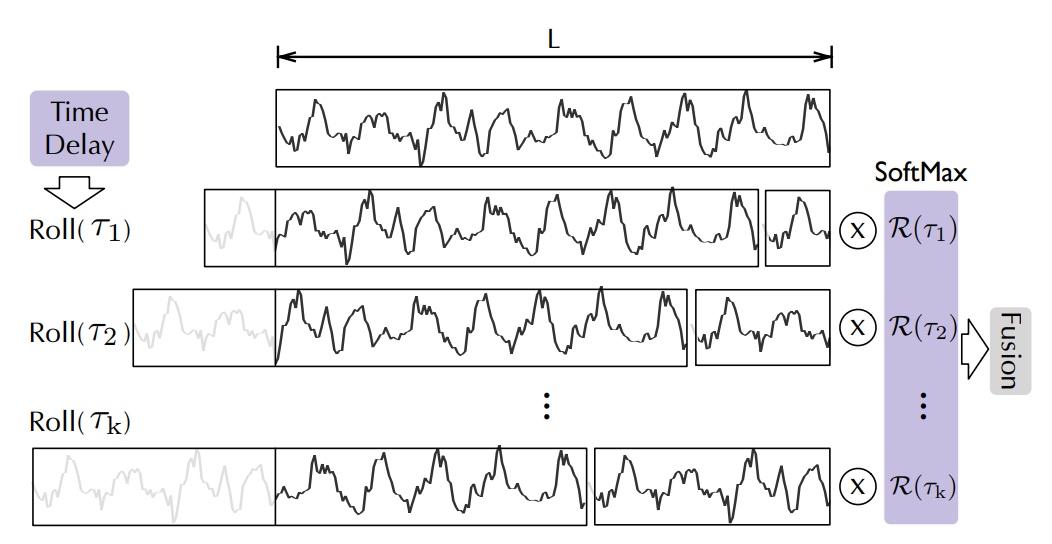
\includegraphics[width=0.6\textwidth]{img/autocorrelation.png}
    \caption{A visualization of autocorrelation module.}
    \label{fig:autocorrelation}
\end{figure}

For efficient computation of $R_{Q, K}(\tau)$, the model employs the Fast Fourier Transforms. 
We refer the interested readers to the original paper for more details. 

\subsection{Experiments}
The experiments are designed to explain the superior performance brought about by the decomposition module and autocorrelation module, respectively, and investigate their robustness under different regularities. 
On top of real-world benchmarks, we generate nine synthetic datasets of various characteristics. 
Except stated explicitly, the models are trained and evaluated under the same hyperparameter setting. 

\subsubsection{Datasets}
To avoid complicating the analysis, all synthetic datasets are univariate ($d = 1$) with the same length, that is, 8k timestamps. 
We take one untrended dataset, \texttt{sinx}, as an example to illustrate the data generation process. 
To begin, we initialize a equally spaced sequence of length 8k: $$X = [\cdots, -0.75, -0.50, -0.25, 0., 0.25, 0.50, 0.75, \cdots].$$
Then, we feed it into some pre-defined function (\texttt{sin} in this case). 
Finally, Gaussian noise with zero mean and appropriate standard deviation is added. 
Importantly, we make the underlying period (if any) so small that the length of the encoder input (see Figure \ref{fig:sinx}) is sufficient to discover periodicity. 

\begin{figure}
    \centering
    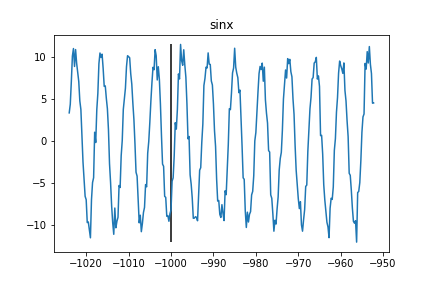
\includegraphics[width=0.5\textwidth]{img/data_sinx.png}
    \caption{A subsequence of the entire \texttt{sinx} dataset. 
    To the left of the black vertical line is fed into the encoder, while to the right is to be predicted. 
    The encoder \textit{should} be able to discover the periodicity.}
    \label{fig:sinx}
\end{figure}

Our synthetic datasets can be categorized into trended (i.e. containing underlying trend) and untrended (i.e. oscilating around 0). 
As for the oscilation, one underlying cycle corresponds to approximately 25 timestamps or length of 6 on the real line. 
Denoting standard Gaussian noise by $\Nc$, we present an overview of different datasets as follows. 
Readers may proceed to Appendix \ref{app:data} for visualizations of all datasets. \begin{itemize}
    \item Trended \begin{itemize}
        \item \texttt{x}: $Y = X + \Nc$. This is just a canonical trend. 
        \item \texttt{sinx\_x}: $Y = 10\sin X + X + \Nc$. It additively combines the canonical trend with a cyclical pattern. Signal-trend decomposition should work well in this case. 
        \item \texttt{sinx\_sqrtx}: $Y = 10\sin X + 20\sqrt{X - \min(X)} + \Nc$. The trend is non-linear and, more specifically, concave downward. 
        \item \texttt{sinx\_x2\_sym}: $Y = 10\sin X + (\frac{X}{50})^2 + \Nc$. The trend is symmetric and concave upward. 
        \item \texttt{sinx\_x2\_asym}: $Y = 10\sin X + (\frac{X - \min(X)}{30})^2 + \Nc$. The trend is assymetric and concave upward. The training and test datasets have drastically different means. 
    \end{itemize}
    \item Untrended \begin{itemize}
        \item \texttt{sinx}: $Y = 10\sin X + \Nc$. This is just a canonical periodic pattern. Autocorrelation module should be able to capture it. 
        \item \texttt{xsinx}: $Y = e^{X \mod 4} \dot (10\sin X + \Nc)$. The amplitude varies over time. 
        \item \texttt{sinx\_sin2x\_sin4x}: $Y = 10\sin X + 10\sin 2X + 10\sin 4X + \Nc$. The periodic pattern is more complicated. 
        \item \texttt{sinx\_c}: $Y = 10\sin X + (-1)^{\mathbb{I}[X \mod 16 < 8]} 30 + \Nc$. Each subsequence is shifted either upward or downward, requiring greater flexibility to capture these drastic changes. 
    \end{itemize}
\end{itemize}

Meanwhile, we also perform ablation studies on the aforementioned real-world datasets. Detailed dataset descriptions can be found in Section \ref{benchmarks}. 

\subsubsection{Results}

According to Figure \ref{fig:trended_mse}, when there is an underlying trend, incorporating decomposition module improves the model performance significantly. 
Instead, if we naively employ autocorrelation module without a proper detrending process, the model can get even more confused. 
On the other hand, if there is no trend in the first place, decomposition module can in fact create negative impacts, possibly by introducing random noise. 

\begin{figure}
    \centering
    \begin{subfigure}{0.6\textwidth}
        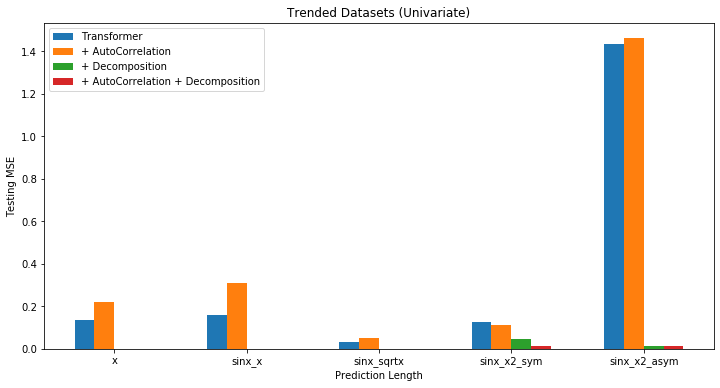
\includegraphics[width=\textwidth]{img/mse_trended.png}
    \end{subfigure}
    \begin{subfigure}{0.6\textwidth}
        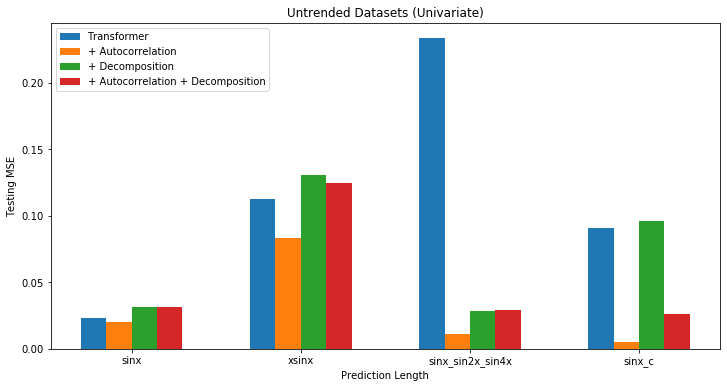
\includegraphics[width=\textwidth]{img/mse_untrended.png}
    \end{subfigure}
    \caption{Mean square errors on trended and untrended synthetic datasets. The \texttt{+ AutoCorrelation + Decomposition} case is equivalent to the Autoformer.}
    \label{fig:trended_mse}
\end{figure}

Figure \ref{fig:synth_pred} plots the forecasting results of a randomly chosen subsequence. 
Plots for other datasets can be found in Appendix \ref{app:pred}. 
As expected, the decomposition module \textit{recalibrate} the prediction baseline to an appropriate level, so the final results would not deviate too much from the target. 

\begin{figure}
    \centering
    \begin{subfigure}{0.9\textwidth}
        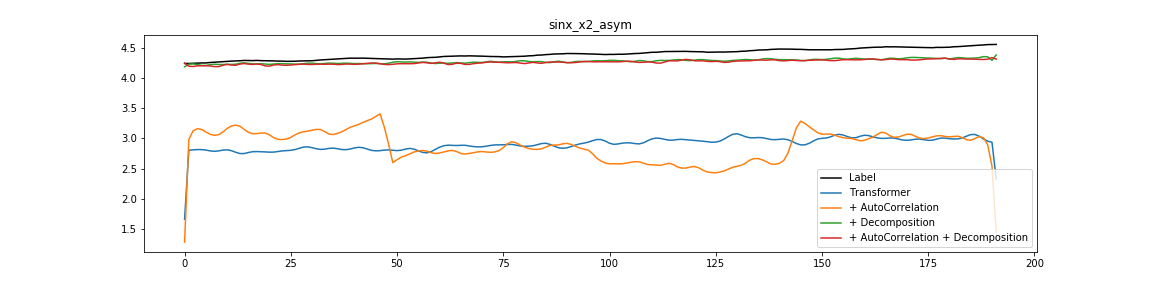
\includegraphics[width=\textwidth]{img/pred_sinx_x2_asym.png}
    \end{subfigure}
    \begin{subfigure}{0.9\textwidth}
        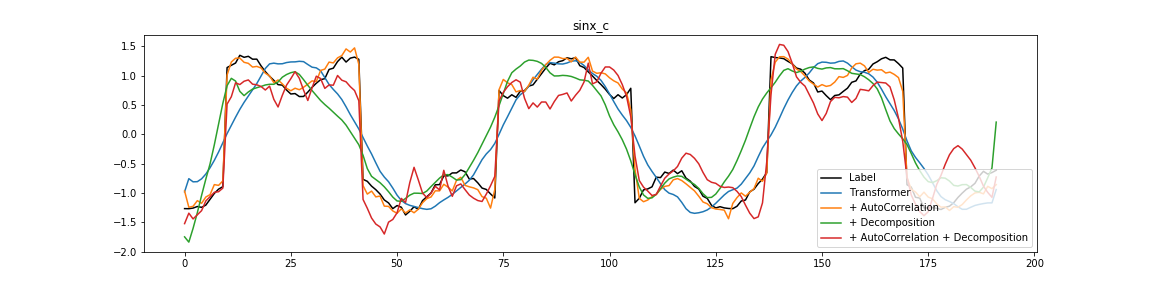
\includegraphics[width=\textwidth]{img/pred_sinx_c.png}
    \end{subfigure}
    \caption{Forecasting plots of a random subsequence in one trended and one untrended synthetic datasets.}
    \label{fig:synth_pred}
\end{figure}

Since decomposition module simply computes the running average, the size of sliding window is a hyperparameter. 
Recall that by construction, one period corresponds to approximately 25 timestamps. 
Thus, we may expect models with sliding window size an integer multiple of 25 to achieve better performance. 
Figure \ref{fig:lwin} indeed confirms our expectation and emphasizes the importance of choosing an appropriate window size. 

As for the autocorrelation module, we notice that as long as the signal has been detrended, it is capable of improving the forecasting quality. 
This phenomenon is especially pronounced when we know beforehand that the data is untrended, so no decopmosition is performed to avoid introducing noise. 

\begin{figure}
    \centering
    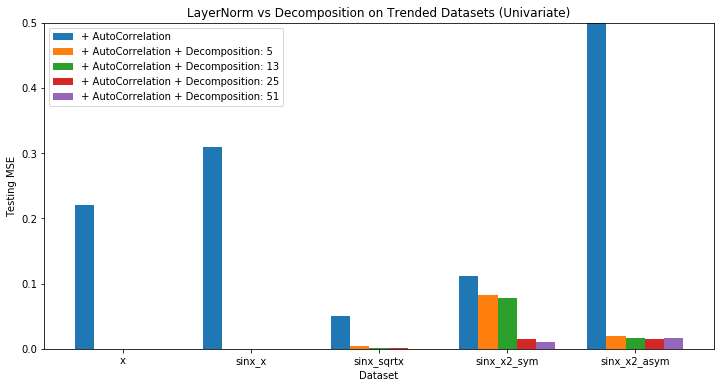
\includegraphics[width=0.6\textwidth]{img/mse_trended_decomp.png}
    \caption{Mean square errors of models with varying decomposition window sizes.}
    \label{fig:lwin}
\end{figure}

Furthermore, we can explore the explainability of autocorrelation weights, just like the attention weights. 
We expect that the top-$k$ most significant $\tau$'s will include an integer multiple of 25 very often. 
Unfortunately, Figure \ref{fig:tau_synth} shows a case where the distribution of $\tau$ does not align with our intuition. 
More examples can be found in Appendix \ref{app:tau}. 
Most of the time, the distribution of $\tau$ does not seem to offer insight into the underlying periodicity of the data. 
Therefore, the working mechanism of the autocorrelation module appears to be a black box awaiting for future discovery. 

\begin{figure}
    \centering
    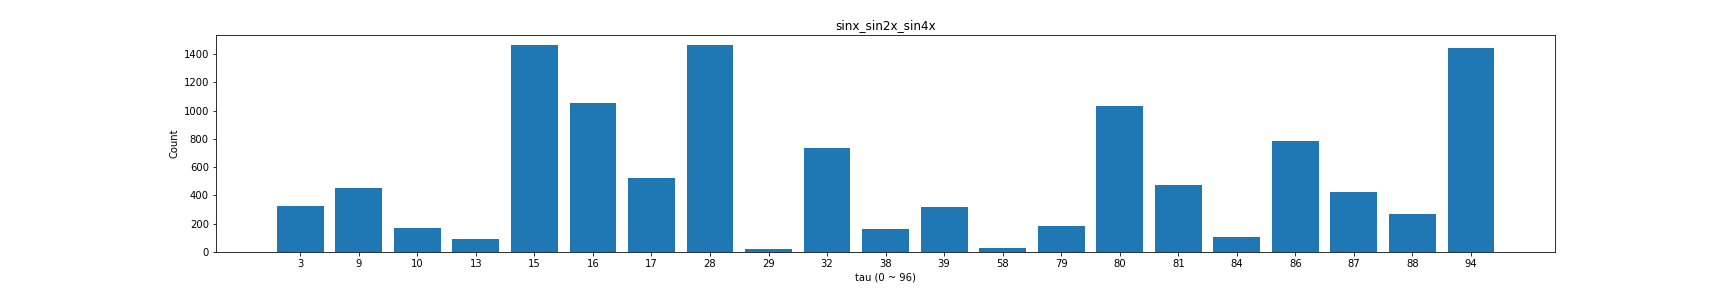
\includegraphics[width=\textwidth]{img/tau_sinx_sin2x_sin4x.png}
    \caption{For each $\tau$, the number of times $R_{Q, K}(\tau)$ is a top-$k$ largest one.}
    \label{fig:tau_synth}
\end{figure}

\begin{figure}
    \centering
    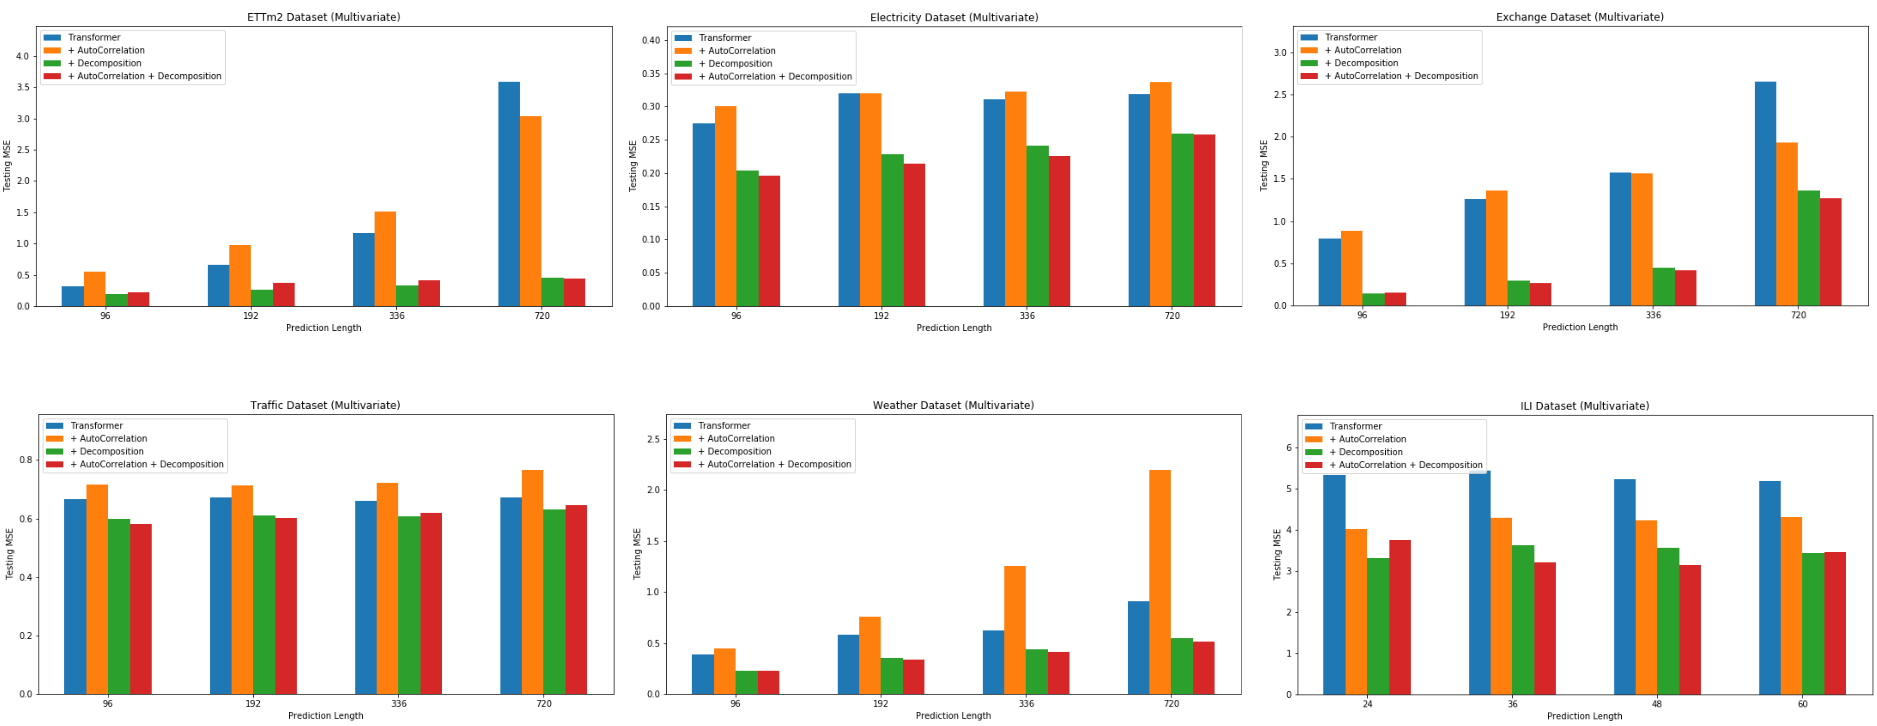
\includegraphics[width=\textwidth]{img/mse_real.png}
    \caption{Mean square errors vanilla Transformer and its variants on real-world datasets.}
    \label{fig:mse_real}
\end{figure}

Finally, we show the results on real-world datasets in Figure \ref{fig:mse_real}. 
The baseline model is vanilla Transformer and we replaces the attention module by autocorrelation module and/or layer normlization module by decomposition module. 
Consistent with findings due to \citet{https://doi.org/10.48550/arxiv.2106.13008}, the greatest empirical improvement comes from the decomposition module. 
However, the effect of autocorrelation module is more nuanced. 
This is possibly because the trend is harder to be identified and removed, and the underlying cyclical patterns are more complicated. 
While harder to interpret, the prediciton plots is also available in Appendix \ref{app:pred}. 



\section{Discussion}
This report reviews the recent progress of using Transformer and its variants on the time series forecasting task. 
In particular, we focus on non-autoregressive decoding, seasonal-trend decomposition module and autocorrelation module, which empirically yields largest performance gains, and conduct comprehensive probing experiemnts to understand their working mechanism. 

Shifting from autoregressive decoding to non-autoregressive decoding retains the original performance. 
That the shift is not as easy in conventional Natural Langauge Processing tasks as in this case may due to different statistical regularities in natural languages and time series. 
Nonetheless, the empirical results suggest non-autoregressive method as a baseline for architectural innovations. 
In contrast, the asymptotic improvement of attention mechanism creates little, if any, speedup, possibly because of the introduced overhead. 

Despite non-parametric and seemingly naive, the decomposition module dramatically improves various Transformers across synthetic and real-world datasets. 
Still, it is not perfect. According to results on the synthetic datasets, this module may introduce noise into inherently clean and non-stationary data; also, it takes a hyperparameter which is hard to determine analytically in real world scenarios. 
With that being said, the ability to recalibrate the level at which predictions are performed makes it a strong baseline. 

Autocorrelation module performs sequence-level attention, replacing the vanilla token-level attention. 
Although it achieves respectable performance gain on untrended synthetic datasets, it is vulnerable to the interference of trended signals. 
Furthermore, the autocorrelation weights lack the explainability as its attention counterpart. 

In conclusion, non-autoregressive decoding is worth to be considered as a baseline approach. 
Besides, Autoformer's successes suggest future work improving the detrending mechanism and enhancing the sequence-level attention's robustness. 


\newpage
\bibliographystyle{plainnat}
\bibliography{reference.bib}


\newpage
\appendix
\section{Synthetic Datasets}\label{app:data}
\begin{figure}[ht]
    \centering
    \begin{subfigure}{0.45\textwidth}
        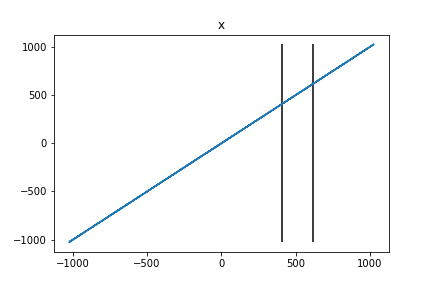
\includegraphics[width=\textwidth]{img/data_x.png}
    \end{subfigure}
    \begin{subfigure}{0.45\textwidth}
        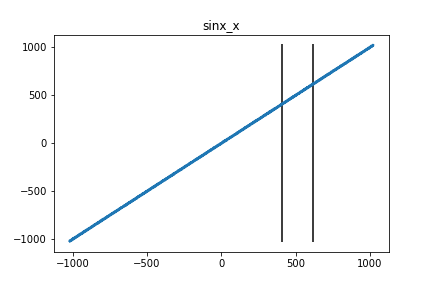
\includegraphics[width=\textwidth]{img/data_sinx_x.png}
    \end{subfigure}
    \begin{subfigure}{0.45\textwidth}
        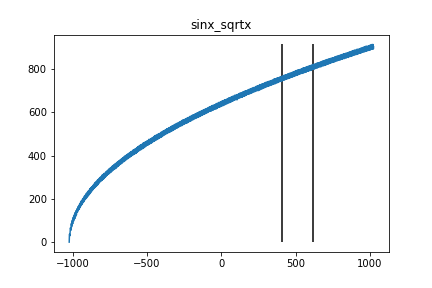
\includegraphics[width=\textwidth]{img/data_sinx_sqrtx.png}
    \end{subfigure}
    \begin{subfigure}{0.45\textwidth}
        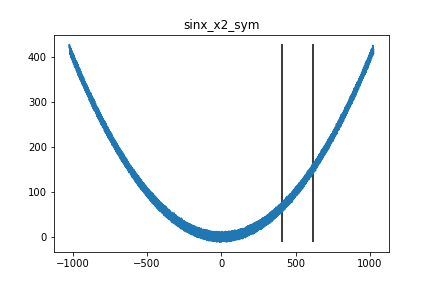
\includegraphics[width=\textwidth]{img/data_sinx_x2_sym.png}
    \end{subfigure}
    \begin{subfigure}{0.45\textwidth}
        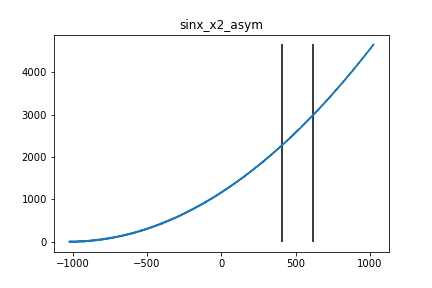
\includegraphics[width=\textwidth]{img/data_sinx_x2_asym.png}
    \end{subfigure}
    \caption{Synthetic datasets with underlying trend. 
    The entire datasets are plotted, so the cyclical patterns by \texttt{sin} function is not visually identifiable. 
    The black vertical lines split the the training, development and test datasets, from left to right.}
\end{figure}

\begin{figure}[ht]
    \centering
    \begin{subfigure}{0.45\textwidth}
        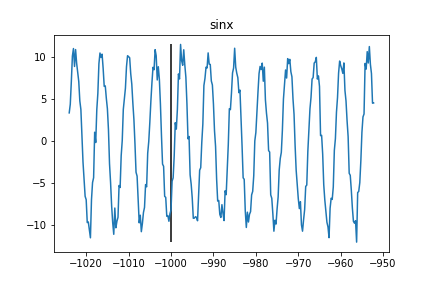
\includegraphics[width=\textwidth]{img/data_sinx.png}
    \end{subfigure}
    \begin{subfigure}{0.45\textwidth}
        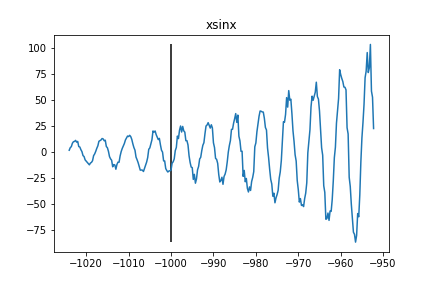
\includegraphics[width=\textwidth]{img/data_xsinx.png}
    \end{subfigure}
    \begin{subfigure}{0.45\textwidth}
        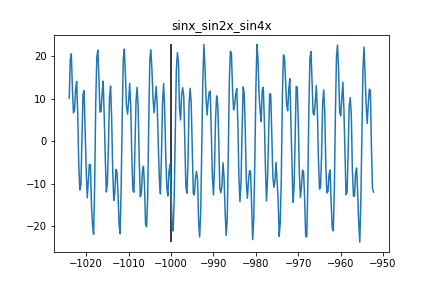
\includegraphics[width=\textwidth]{img/data_sinx_sin2x_sin4x.png}
    \end{subfigure}
    \begin{subfigure}{0.45\textwidth}
        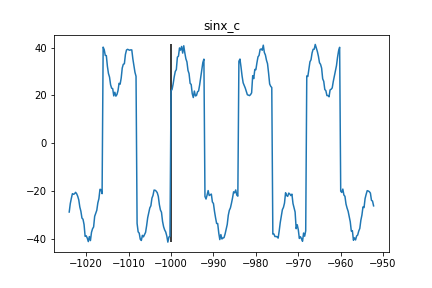
\includegraphics[width=\textwidth]{img/data_sinx_c.png}
    \end{subfigure}
    \caption{Synthetic datasets without underlying trend. 
    Only one subsequence is plotted, where the black vertical line splits the encoder input and forecasting target.}
\end{figure}
\clearpage


\section{Prediction Plots}\label{app:pred}
\begin{figure}[ht]
    \centering
    \begin{subfigure}{0.75\textwidth}
        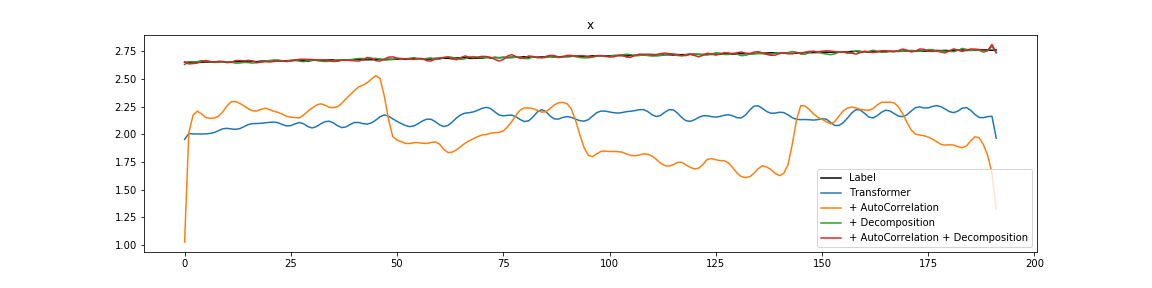
\includegraphics[width=\textwidth]{img/pred_x.png}
    \end{subfigure}
    \begin{subfigure}{0.75\textwidth}
        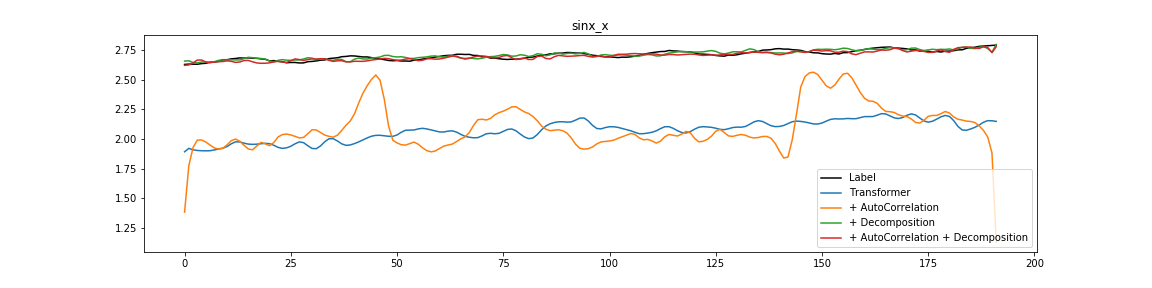
\includegraphics[width=\textwidth]{img/pred_sinx_x.png}
    \end{subfigure}
    \begin{subfigure}{0.75\textwidth}
        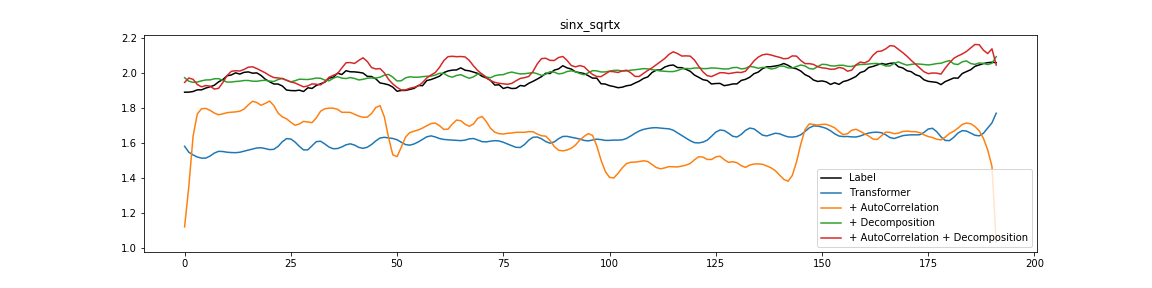
\includegraphics[width=\textwidth]{img/pred_sinx_sqrtx.png}
    \end{subfigure}
    \begin{subfigure}{0.75\textwidth}
        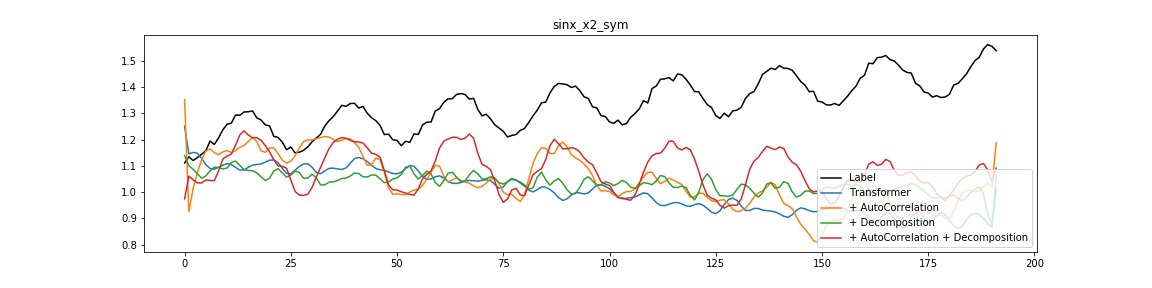
\includegraphics[width=\textwidth]{img/pred_sinx_x2_sym.png}
    \end{subfigure}
    \begin{subfigure}{0.75\textwidth}
        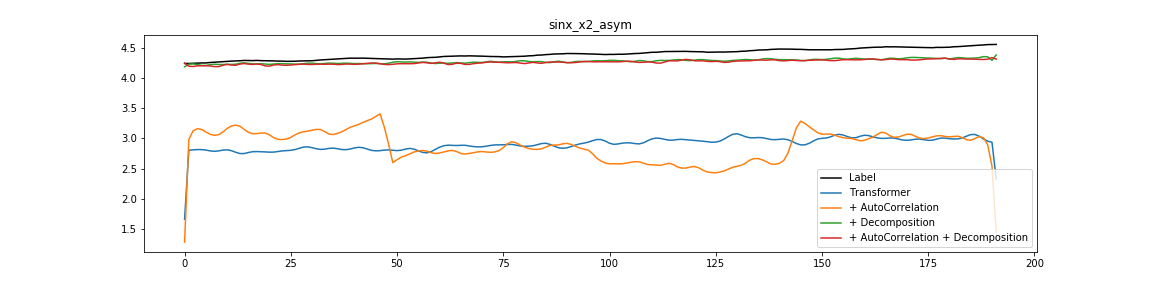
\includegraphics[width=\textwidth]{img/pred_sinx_x2_asym.png}
    \end{subfigure}
    \caption{Forecasting one subsequence in synthetic datasets with underlying trend.}
\end{figure}

\begin{figure}[ht]
    \centering
    \begin{subfigure}{0.75\textwidth}
        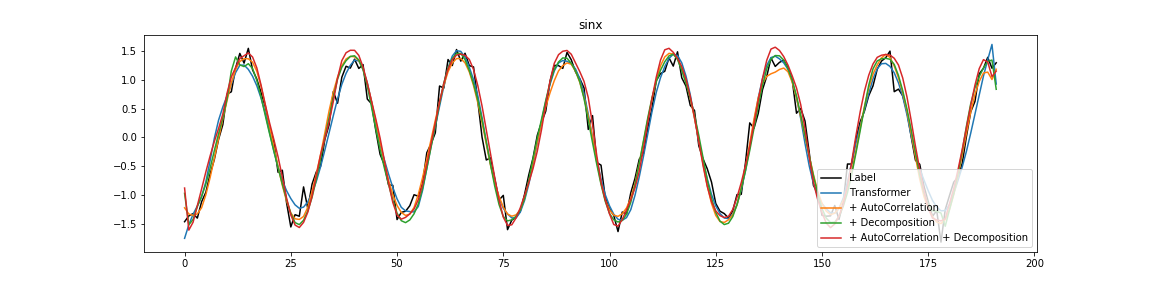
\includegraphics[width=\textwidth]{img/pred_sinx.png}
    \end{subfigure}
    \begin{subfigure}{0.75\textwidth}
        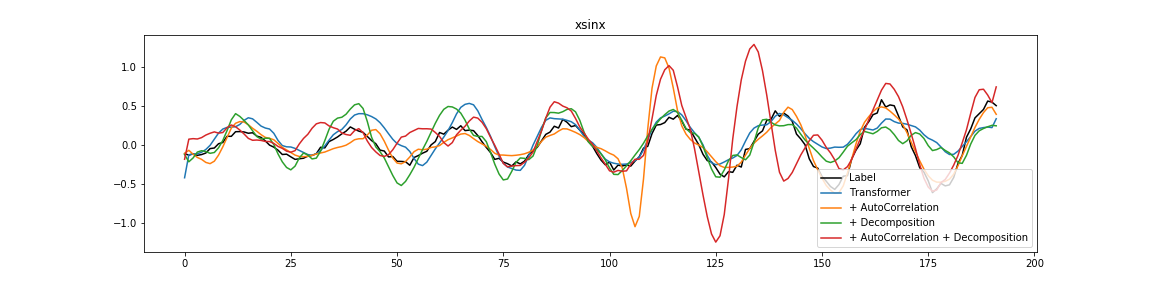
\includegraphics[width=\textwidth]{img/pred_xsinx.png}
    \end{subfigure}
    \begin{subfigure}{0.75\textwidth}
        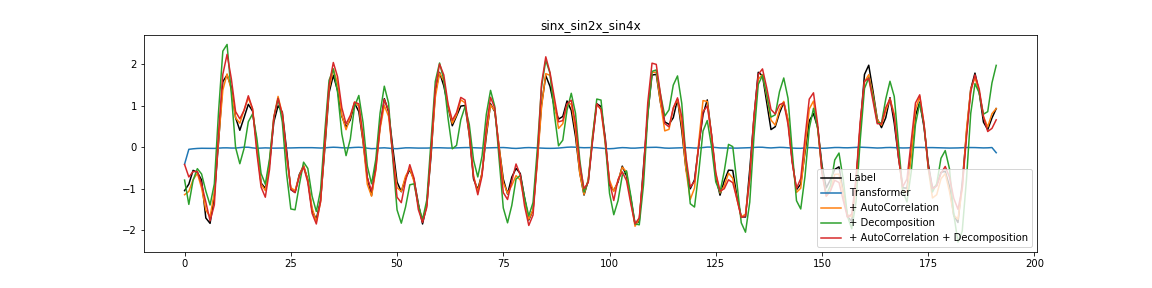
\includegraphics[width=\textwidth]{img/pred_sinx_sin2x_sin4x.png}
    \end{subfigure}
    \begin{subfigure}{0.75\textwidth}
        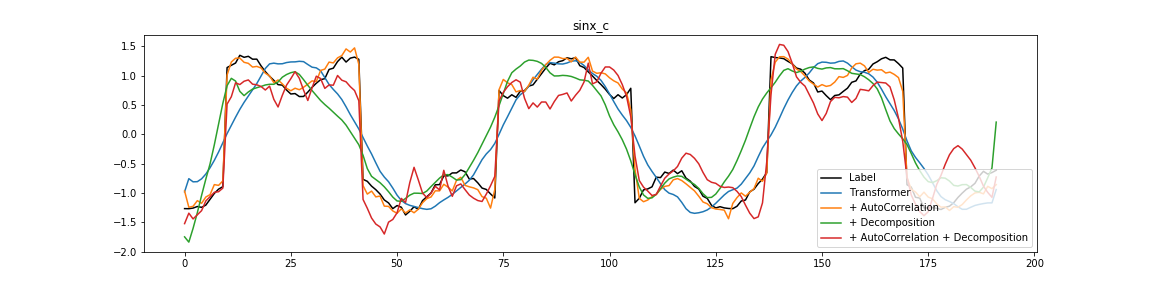
\includegraphics[width=\textwidth]{img/pred_sinx_c.png}
    \end{subfigure}
    \caption{Forecasting one subsequence in synthetic datasets without underlying trend.}
\end{figure}

\begin{figure}[ht]
    \centering
    \begin{subfigure}{0.6\textwidth}
        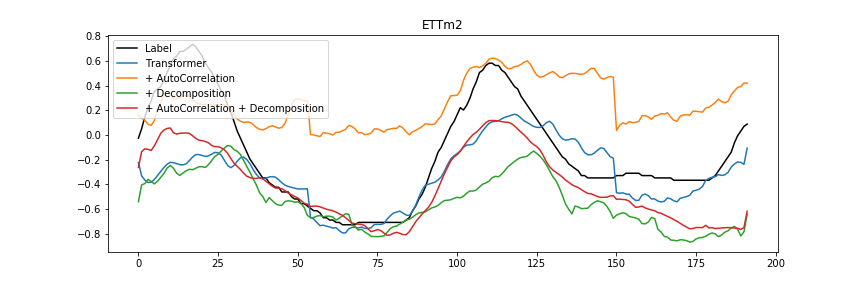
\includegraphics[width=\textwidth]{img/pred_ETTm2.png}
    \end{subfigure}
    \begin{subfigure}{0.6\textwidth}
        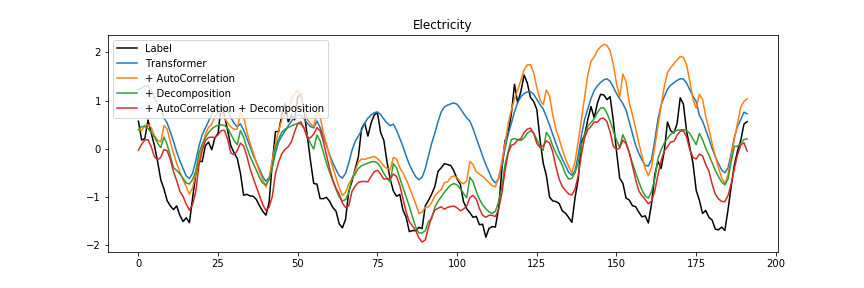
\includegraphics[width=\textwidth]{img/pred_Electricity.png}
    \end{subfigure}
    \begin{subfigure}{0.6\textwidth}
        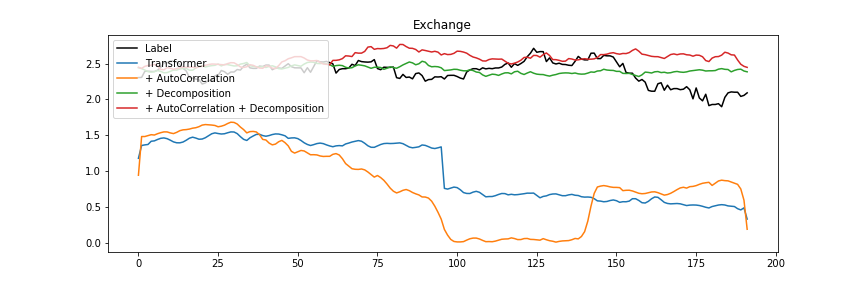
\includegraphics[width=\textwidth]{img/pred_Exchange.png}
    \end{subfigure}
    \begin{subfigure}{0.6\textwidth}
        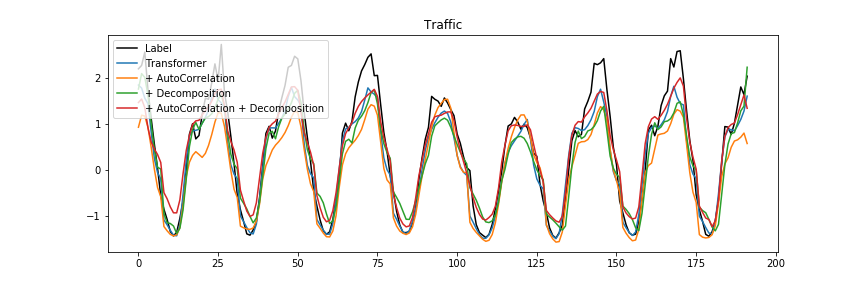
\includegraphics[width=\textwidth]{img/pred_Traffic.png}
    \end{subfigure}
    \begin{subfigure}{0.6\textwidth}
        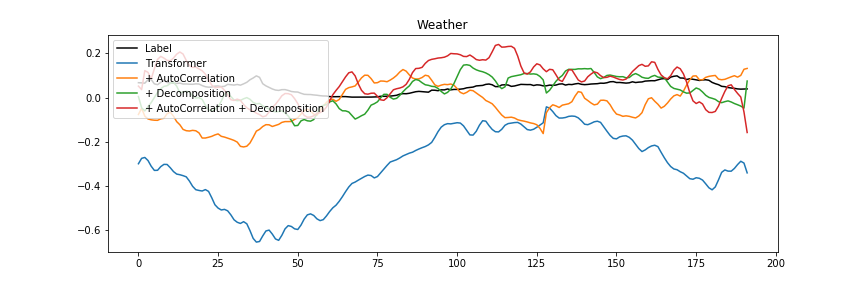
\includegraphics[width=\textwidth]{img/pred_Weather.png}
    \end{subfigure}
    \begin{subfigure}{0.6\textwidth}
        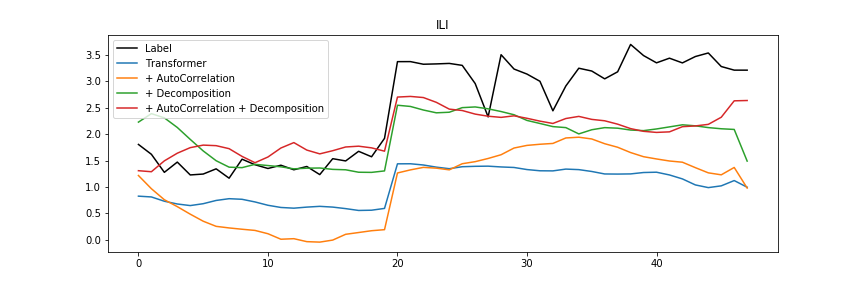
\includegraphics[width=\textwidth]{img/pred_ILI.png}
    \end{subfigure}
    \caption{Forecasting one subsequence in synthetic datasets without underlying trend.}
\end{figure}
\clearpage


\section{AutoCorrelation Weights}\label{app:tau}
\begin{figure}[ht]
    \centering
    \begin{subfigure}{\textwidth}
        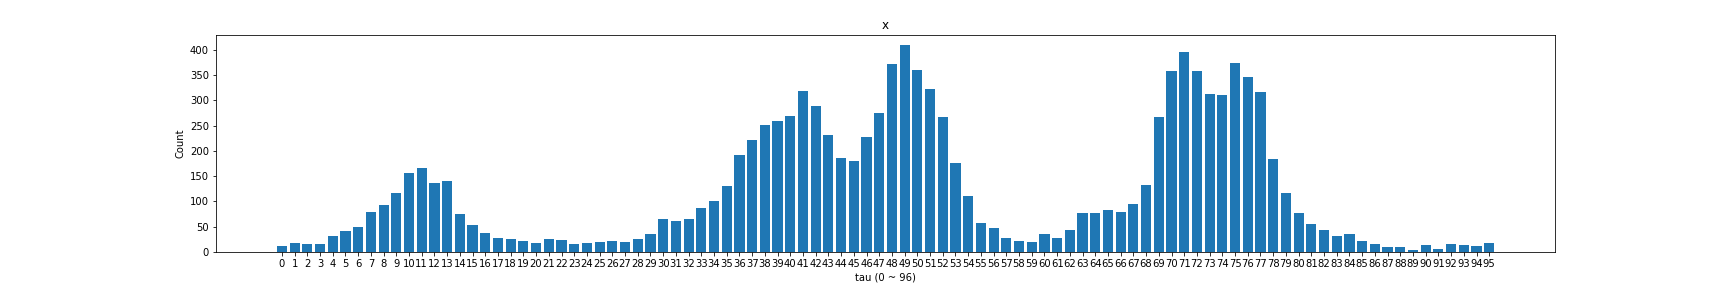
\includegraphics[width=\textwidth]{img/tau_x.png}
    \end{subfigure}
    \begin{subfigure}{\textwidth}
        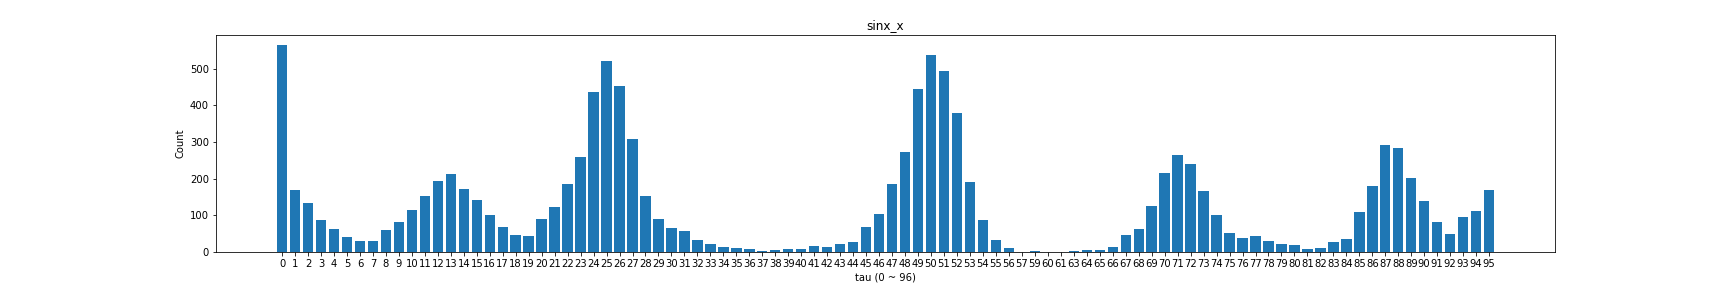
\includegraphics[width=\textwidth]{img/tau_sinx_x.png}
    \end{subfigure}
    \begin{subfigure}{\textwidth}
        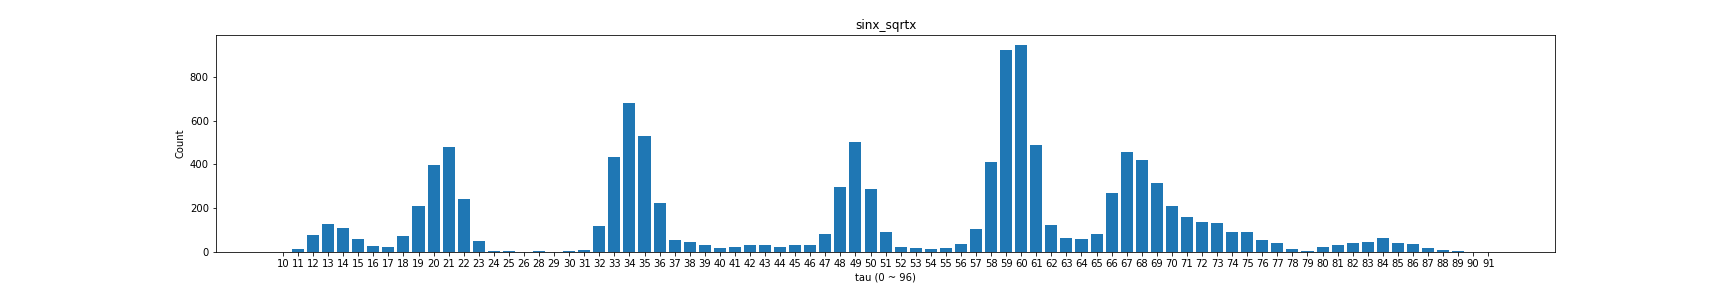
\includegraphics[width=\textwidth]{img/tau_sinx_sqrtx.png}
    \end{subfigure}
    \begin{subfigure}{\textwidth}
        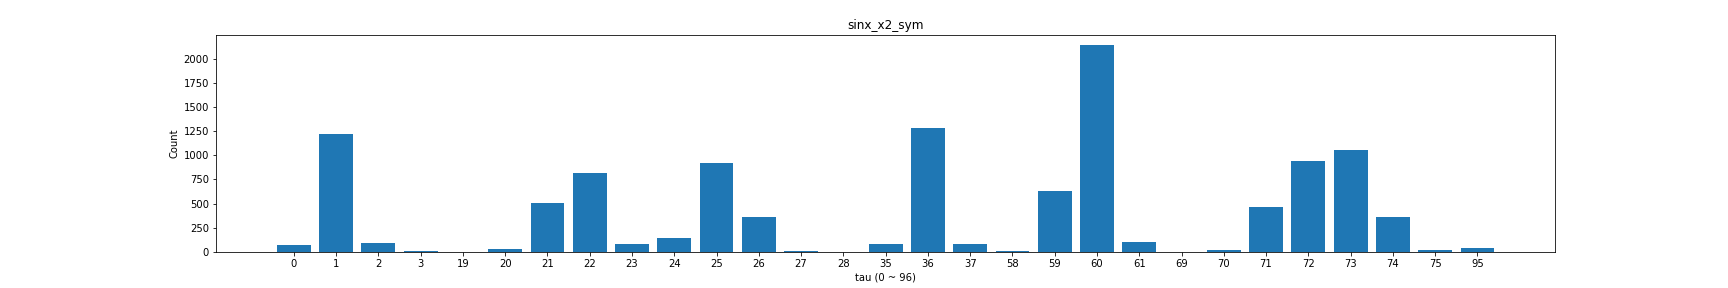
\includegraphics[width=\textwidth]{img/tau_sinx_x2_sym.png}
    \end{subfigure}
    \begin{subfigure}{\textwidth}
        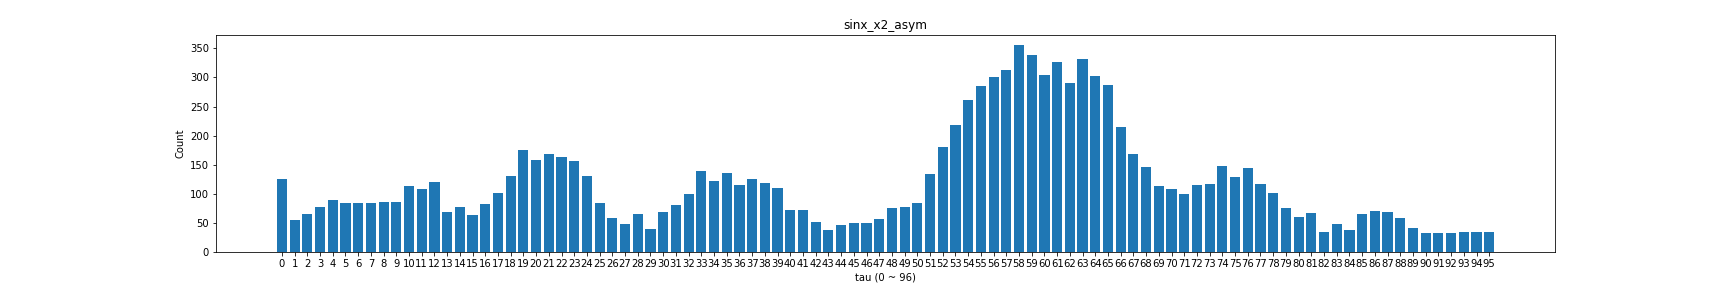
\includegraphics[width=\textwidth]{img/tau_sinx_x2_asym.png}
    \end{subfigure}
    \caption{Distributions of $\tau$ on synthetic datasets with trend.}
\end{figure}

\begin{figure}[ht]
    \centering
    \begin{subfigure}{\textwidth}
        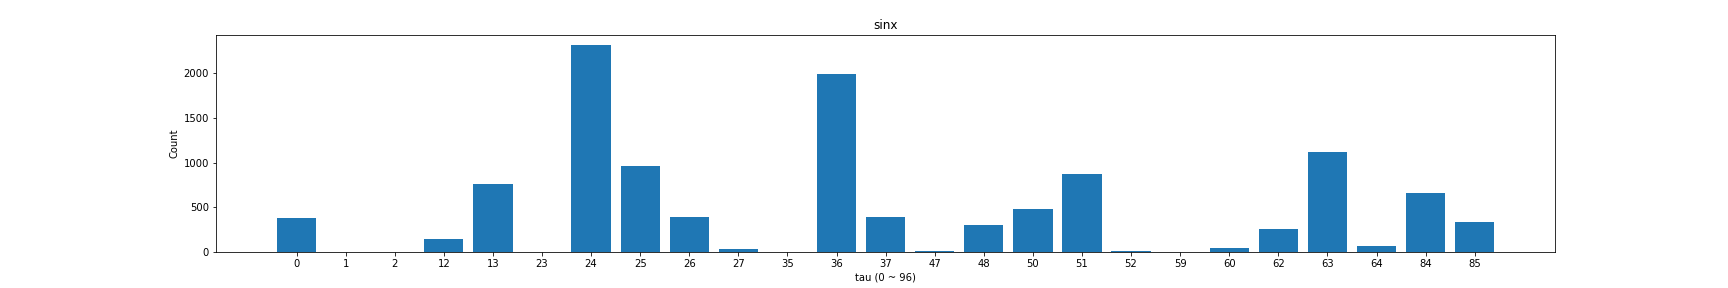
\includegraphics[width=\textwidth]{img/tau_sinx.png}
    \end{subfigure}
    \begin{subfigure}{\textwidth}
        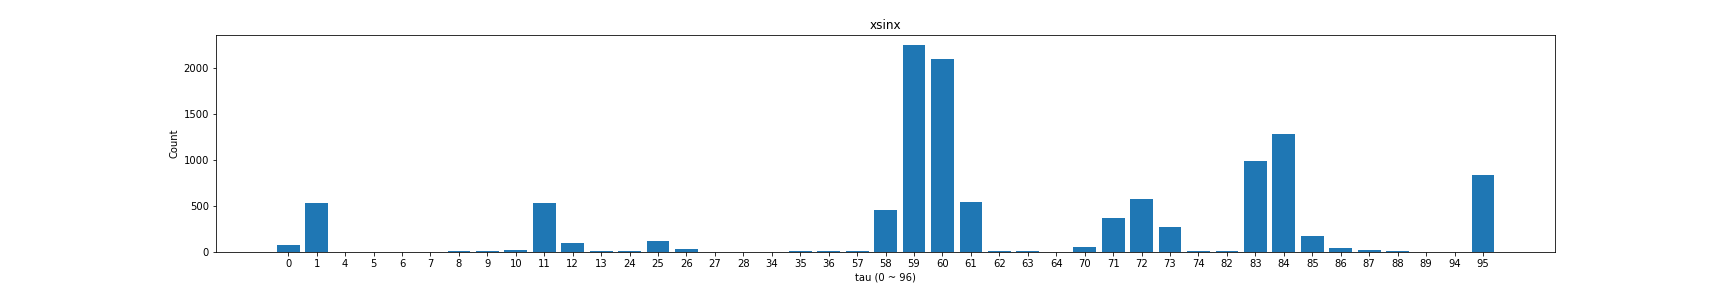
\includegraphics[width=\textwidth]{img/tau_xsinx.png}
    \end{subfigure}
    \begin{subfigure}{\textwidth}
        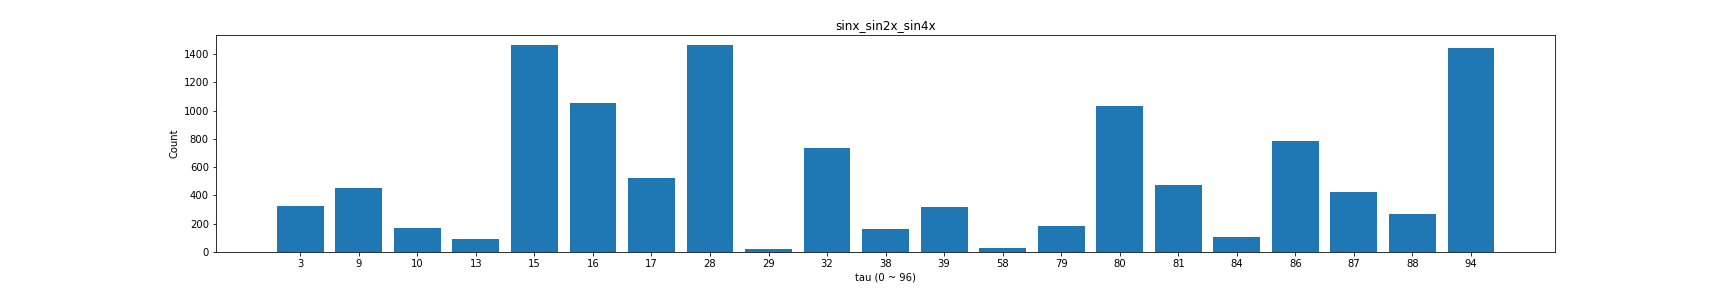
\includegraphics[width=\textwidth]{img/tau_sinx_sin2x_sin4x.png}
    \end{subfigure}
    \begin{subfigure}{\textwidth}
        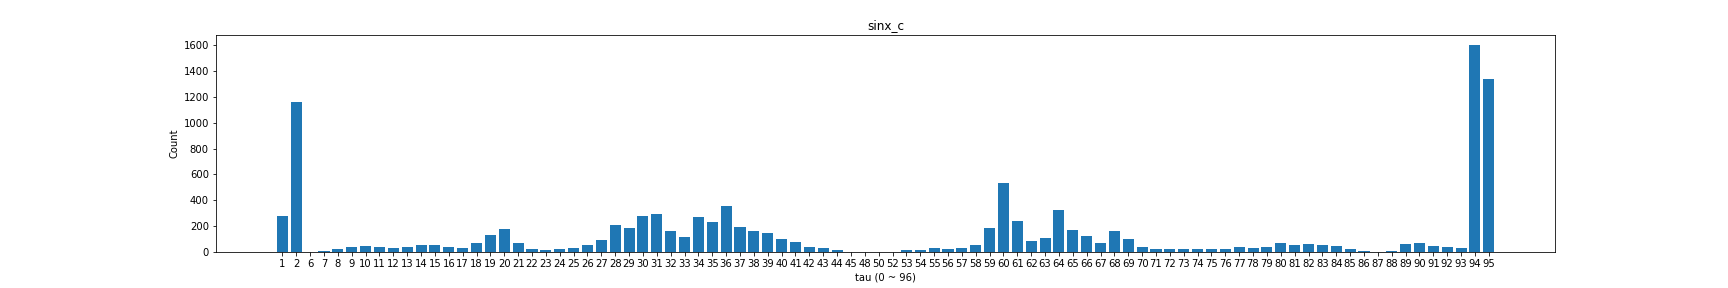
\includegraphics[width=\textwidth]{img/tau_sinx_c.png}
    \end{subfigure}
    \caption{Distributions of $\tau$ on synthetic datasets without trend.}
\end{figure}

\end{document}
